\documentclass{article}

\usepackage{graphicx}
\usepackage{fancyhdr}
\usepackage[sorting=none]{biblatex}
\usepackage[margin=1in]{geometry}
\usepackage{listings}
\usepackage[hidelinks]{hyperref}
\usepackage{xcolor}
\usepackage{xepersian}
\usepackage{ltablex}
\usepackage{booktabs, makecell, longtable}



\addbibresource{bibliography.bib}
\settextfont[Scale=1.2]{IRNazli.ttf}
\setlatintextfont[Scale=1]{times.ttf}
\renewcommand{\baselinestretch}{1.5}
\pagestyle{fancy}
\fancyhf{}
\renewcommand{\headrulewidth}{1pt}
\renewcommand{\footrulewidth}{1pt}
\setcounter{tocdepth}{1}
\begin{document}

\def\by{نگارش}
\def\superv{مدرس}
\def\faculty{دانشکده مهندسی کامپیوتر}
\def\course{رایانش عصبی}
\def\docTitle{پروژه سوم }
\def\supervisor{دکتر رضا صفابخش}
\def\fname{سیدمهدی }
\def\lname{میرفندرسکی}
\def\stuNum{401131065}
\def\docDate{آذر 1401}

\rhead{\docTitle}
\lhead{درس \course}
\rfoot{\fname \lname}
\lfoot{\stuNum}
\cfoot{\\ \thepage}



\begin{titlepage}
\begin{center}
%
\includegraphics[width=0.4\textwidth]{fa-logo.png}\\
\centerline{{
\includegraphics[height=3.8cm]{fa-logo}}}        
\LARGE
%\textbf{دانشگاه صنعتی اصفهان}\\
%\textbf{دانشکده مهندسی کامپیوتر}\\
\bf{\fontsize{16pt}{16pt}\selectfont دانشگاه صنعتی امیرکبیر}\par
\fontsize{14pt}{15pt}\selectfont(پلی‌تکنیک تهران)\par
\fontsize{16pt}{17pt}\selectfont \faculty \par
        
\par
        

\vfill
{\huge\settextfont{B_Titr.ttf}{\docTitle  درس  \course}}
\vfill
 
\settextfont[Scale=1.2]{BNazanin.ttf}
{\huge\by}\\
\fontsize{18pt}{19pt}\selectfont\bfseries{\fname \lname} \\
\settextfont[Scale=1.2]{BNazanin.ttf}
{\huge\superv}\\
{\fontsize{18pt}{19pt}\selectfont\bfseries\par\supervisor}\\
\fontsize{16pt}{17pt}\selectfont\docDate\\
 
 
        
\LARGE
%\textbf{نام و نام خانوادگی: مجید فرهادی}\\
%\textbf{شماره دانشجویی: 9700000}\\
%\textbf{نیم‌سال تحصیلی: پاییز 1400}\\
%\textbf{مدرّس: دکتر محمّدرضا حیدرپور}\\
%\textbf{دستیاران آموزشی: مجید فرهادی - دانیال مهرآیین - محمّد نعیمی}\\
\end{center}
\end{titlepage}


\tableofcontents

\newpage



\section{سوال اول - الف}

ابتدا داده ورودی را در تصویر زیر مشاهده می‌کنیم. هدف بازسازی سطح تصویر سه بعدی یک خرگوش است. برای این کار، یک شبکه دوبعدی با همسایگی مربعی ساده استفاده شد. 

\begin{figure}[!h]
    \centering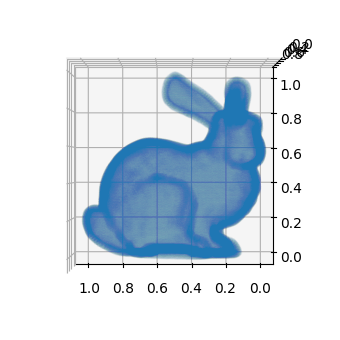
\includegraphics[scale=.55]{./p1-1}
    \caption{تصویر اولیه خرگوش}\label{fig.11}
\end{figure}


\cleardoublepage
در ابتدا شعاع همسایگی مطابق با مطالب گفته شده مقادیر بسیار بزرگتر از 2 قرار داده می‌شد، اما با مشورتی که انجام شد مقدار سیگما (شعاع همسایگی) برابر با 2 گذاشته شد و نتایج بسیار مطلوب‌تری گرفته شد. در زیر نمونه‌هایی از تست‌ها دیده می‌شود (در هر تصویر مشخصات شبکه آموزش داده شده وجود دارد.). لازم به ذکر است که وزن‌های اولیه از خود داده‌ها به صورت تصدفی انتخاب شدند.


\begin{figure}[!h]
    \centering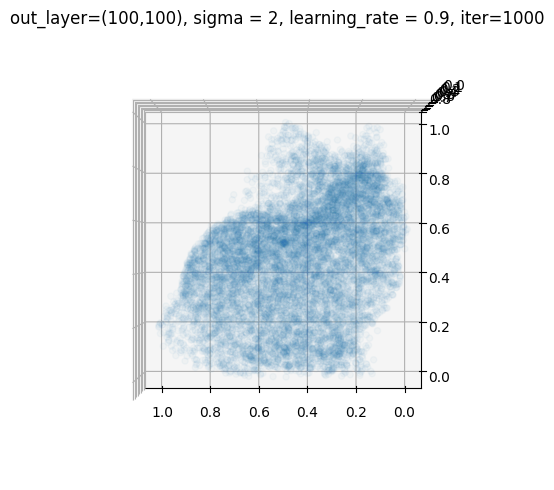
\includegraphics[scale=.65]{./p1-2}
    \caption{تست انجام شده با مشخصات داخل تصویر}\label{fig.12}
\end{figure}


\begin{figure}[!h]
    \centering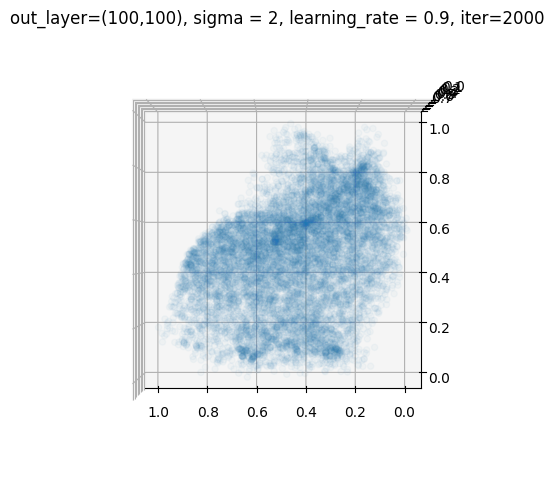
\includegraphics[scale=.65]{./p1-3}
    \caption{تست انجام شده با مشخصات داخل تصویر}\label{fig.13}
\end{figure}

\begin{figure}[!h]
    \centering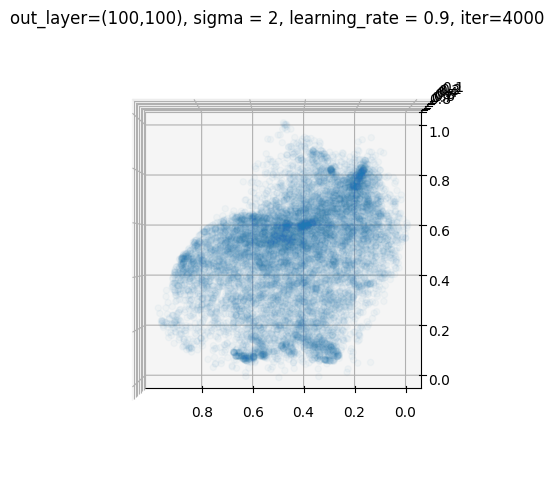
\includegraphics[scale=.65]{./p1-4}
    \caption{تست انجام شده با مشخصات داخل تصویر}\label{fig.14}
\end{figure}

\begin{figure}[!h]
    \centering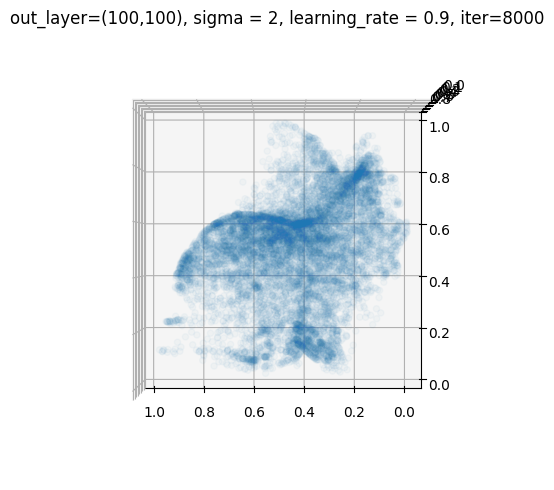
\includegraphics[scale=.65]{./p1-5}
    \caption{تست انجام شده با مشخصات داخل تصویر}\label{fig.15}
\end{figure}

\begin{figure}[!h]
    \centering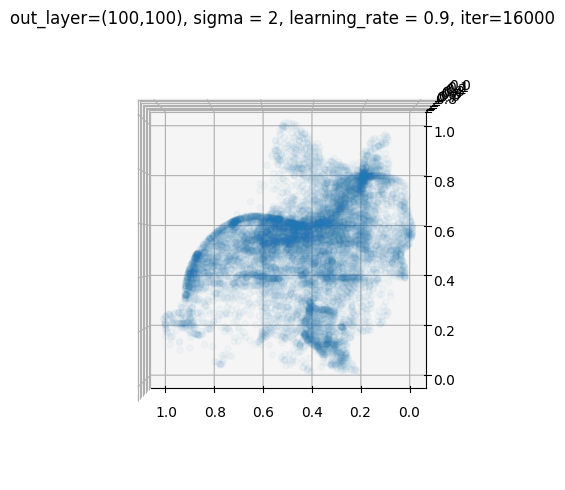
\includegraphics[scale=.65]{./p1-6}
    \caption{تست انجام شده با مشخصات داخل تصویر}\label{fig.16}
\end{figure}

\begin{figure}[!h]
    \centering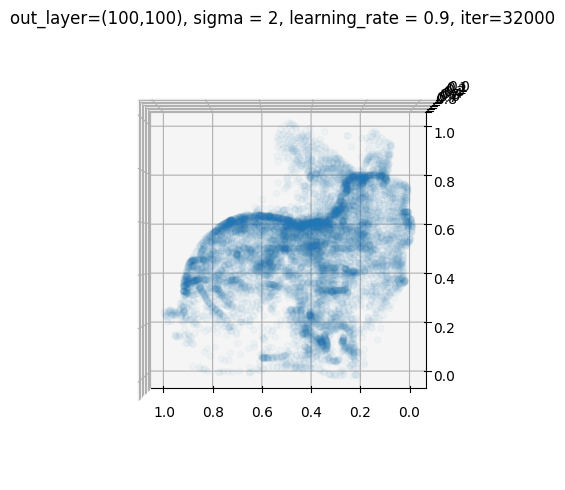
\includegraphics[scale=.65]{./p1-7}
    \caption{تست انجام شده با مشخصات داخل تصویر}\label{fig.17}
\end{figure}

\begin{figure}[!h]
    \centering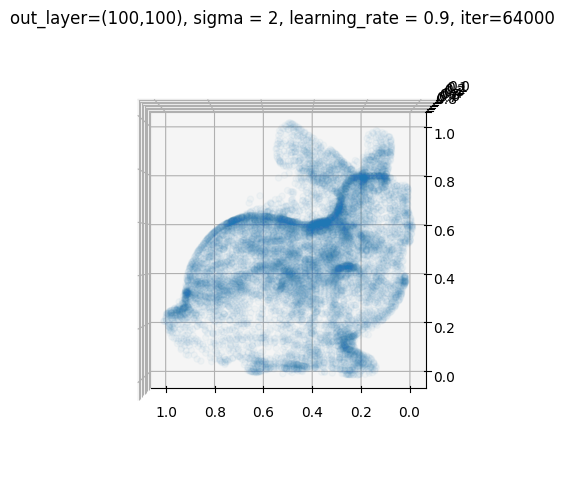
\includegraphics[scale=.65]{./p1-8}
    \caption{تست انجام شده با مشخصات داخل تصویر}\label{fig.18}
\end{figure}

\begin{figure}[!h]
    \centering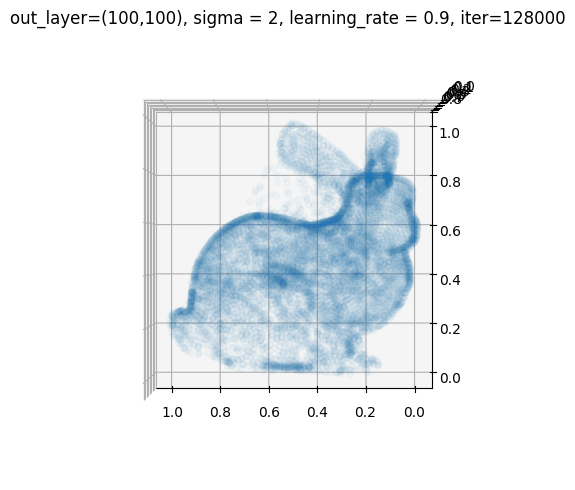
\includegraphics[scale=.65]{./p1-9}
    \caption{تست انجام شده با مشخصات داخل تصویر}\label{fig.19}
\end{figure}

\begin{figure}[!h]
    \centering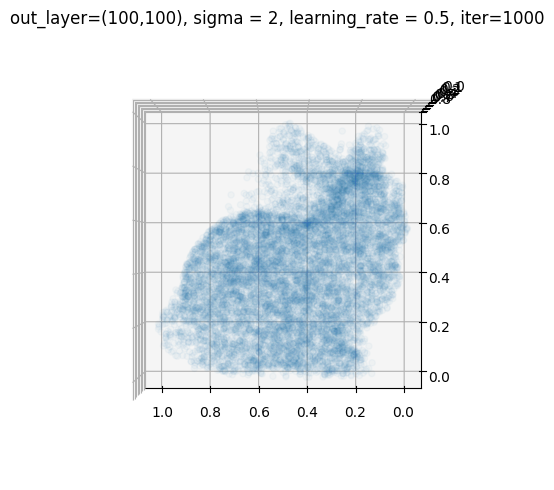
\includegraphics[scale=.65]{./p1-10}
    \caption{تست انجام شده با مشخصات داخل تصویر}\label{fig.110}
\end{figure}

\begin{figure}[!h]
    \centering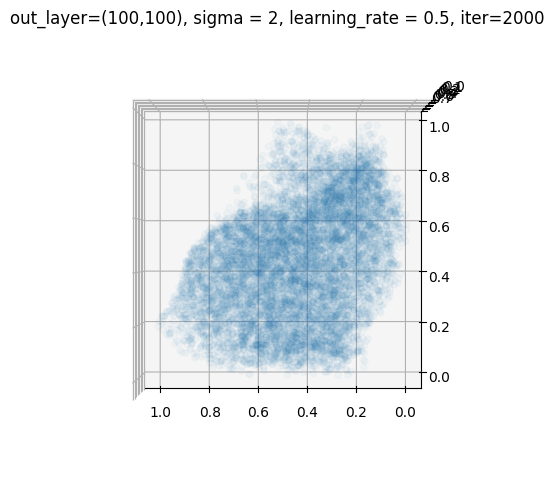
\includegraphics[scale=.65]{./p1-11}
    \caption{تست انجام شده با مشخصات داخل تصویر}\label{fig.111}
\end{figure}

\begin{figure}[!h]
    \centering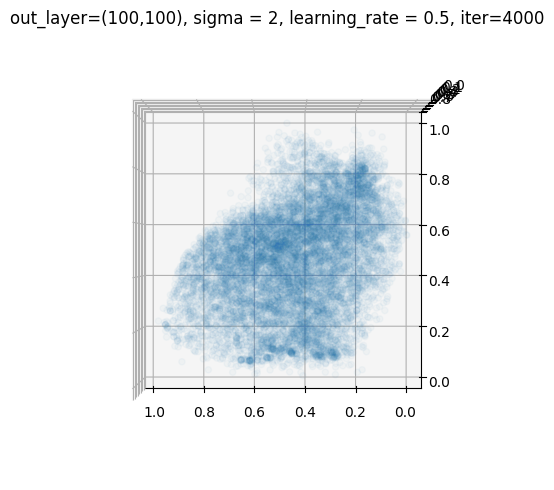
\includegraphics[scale=.65]{./p1-12}
    \caption{تست انجام شده با مشخصات داخل تصویر}\label{fig.112}
\end{figure}

\begin{figure}[!h]
    \centering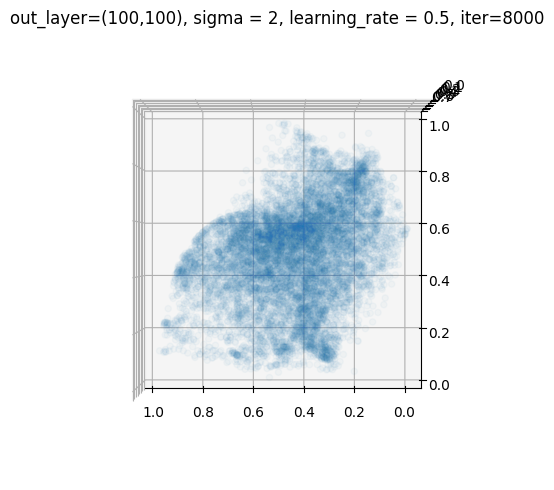
\includegraphics[scale=.65]{./p1-13}
    \caption{تست انجام شده با مشخصات داخل تصویر}\label{fig.113}
\end{figure}

\begin{figure}[!h]
    \centering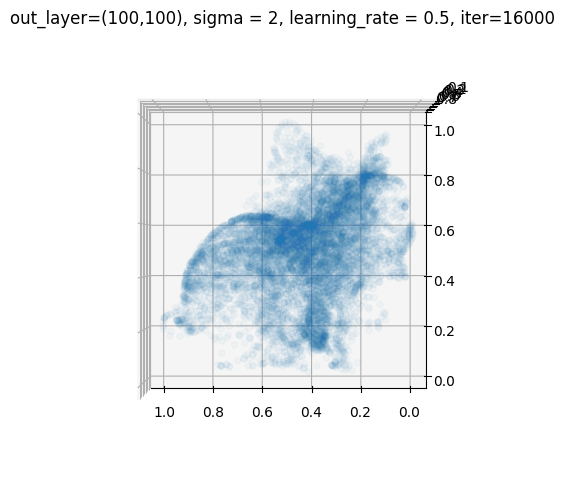
\includegraphics[scale=.65]{./p1-14}
    \caption{تست انجام شده با مشخصات داخل تصویر}\label{fig.114}
\end{figure}

\begin{figure}[!h]
    \centering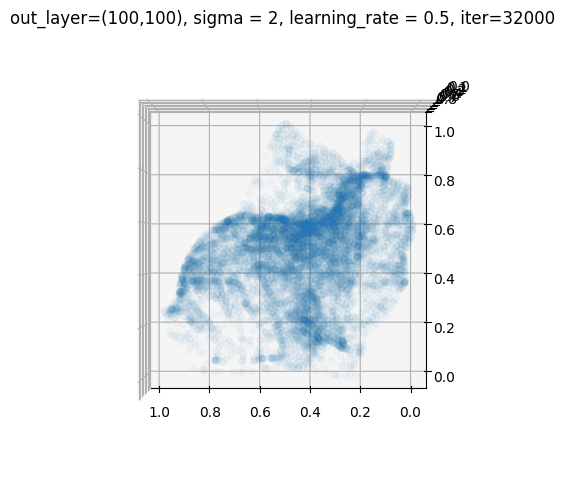
\includegraphics[scale=.65]{./p1-15}
    \caption{تست انجام شده با مشخصات داخل تصویر}\label{fig.115}
\end{figure}

\begin{figure}[!h]
    \centering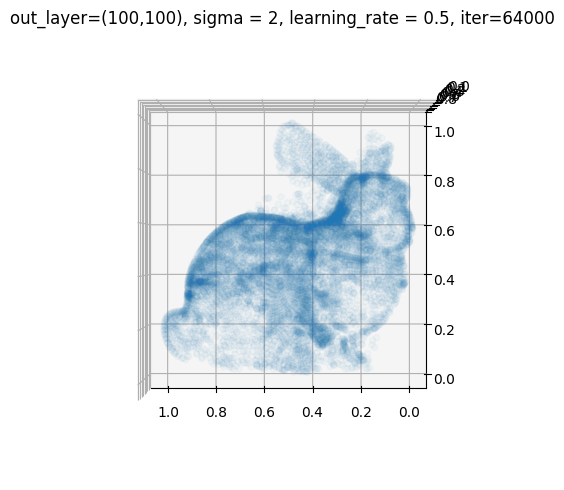
\includegraphics[scale=.65]{./p1-16}
    \caption{تست انجام شده با مشخصات داخل تصویر}\label{fig.116}
\end{figure}

\begin{figure}[!h]
    \centering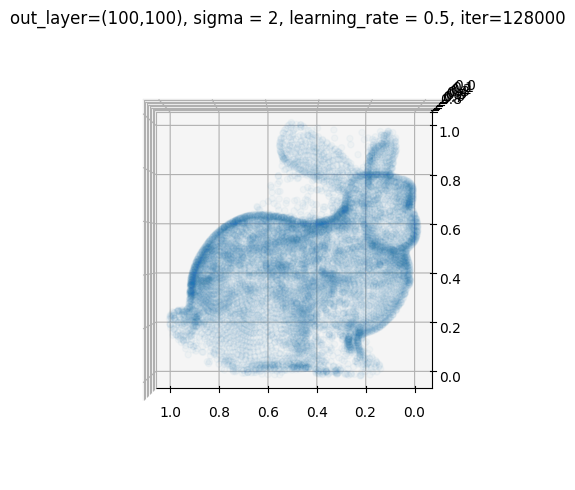
\includegraphics[scale=.65]{./p1-17}
    \caption{تست انجام شده با مشخصات داخل تصویر}\label{fig.117}
\end{figure}


\cleardoublepage

همانطور که دیده می‌شود هرچه تعداد تکرار بیشتر باشد، بازنمایی دقیق‌تری از تصویر اولیه خواهیم داشت. بدین منظور برای شبکه نهایی آموزش داده شد و نتیجه آن در ادامه آمده است.

همانطور که دیده می‌شود، نتیجه آخر نتیجه مطلوبی هست زیرا با توجه به تصویر اولیه به صورت یکنواخت خروجی پخش شده است.

\begin{figure}[!h]
    \centering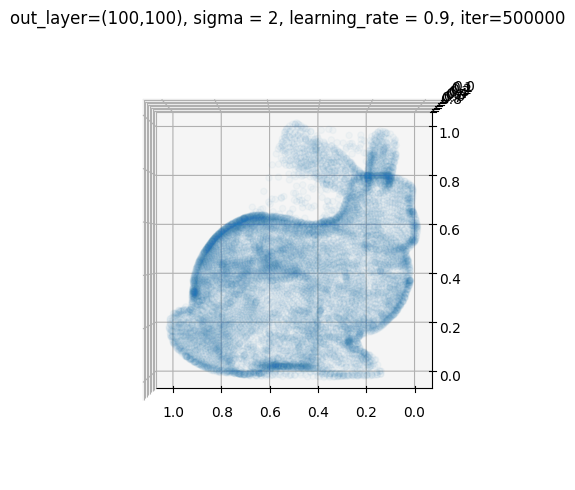
\includegraphics[scale=.65]{./p1-18}
    \caption{تست انجام شده با مشخصات داخل تصویر}\label{fig.118}
\end{figure}

\cleardoublepage

% -------------------------------------------------------------------
\section{سوال اول - ب}

برای این مسئله که بازنمایی سطح یک جسم سه بعدی است، بهتر است لبه‌ها نیز با لبه‌های دیگر همسایه شوند. به نظرم اگر بتوان شبکه‌ای کروی و یا حتی مکعبی (سه بعدی) طراحی کرد، خروجی بهتری حاصل شود. در لبه‌های شبکه دو بعدی همسایگی تضعیف میشود و اگر ما به دنبال بازنمایی سطح هستیم، همسایگی در تمام جهات کمک خواهد کرد و دقت بهتری بدست می‌آید. به بیان دیگر تصویر سه بعدی در لبه‌ها در ممکن است در جهت \lr{x,y} همسایه‌ای نداشته باشند اما در جهت \lr{z} همسایه‌ها وجود خواهند داشت.


% -------------------------------------------------------------------
\section{سوال دوم - الف}

دو خروجی بصری متداول شبکه خودسازمانده ماتریس یو و هیت‌مپ است.

\begin{itemize}
    \item ماتریس یو: فاصله بین هر گره و همسایگان آن به طور معمول با یک پالت خاکستری نمایش داده می‌شود، مناطق با فاصله کم از همسایه‌ها نشان دهنده گروه‌هایی از گره‌ها هستند که مشابه هم هستند. مناطق با فواصل زیاد نیز نشان می‌دهد که گره‌ها بسیار متفاوت‌تر هستند (نشان دهنده مرزها بین خوشه‌های گره). ماتریس یو می‌تواند برای شناسایی خوشه‌ها در شبکه خودسازمانده استفاده شود.
    \item هیت‌مپ: هیت‌مپ شاید مهمترین تجسم ممکن برای نقشه های خودسازمانده باشد. برای یک شبکه با ابعاد بالا (7 متغیر به بالا) نامناسب است. امکان تجسم توزیع یک متغیر را در سراسر نقشه فراهم می‌کند. درواقع مقایسه هیت‌مپ‌های مختلف برای متغیرها مناطق جالب روی نقشه را شناسایی می‌کند. 
    \item خروجی می‌تواند یک تقریب گسسته از توزیع نمونه‌های آموزشی را تشکیل دهند. داده‌های آموزشی شبیه به هم و زیاد بیشتر در خروجی نمود پیدا می‌کنند و بالعکس. لذا این شبکه می‌تواند تعمیم غیرخطی تجزیه و تحلیل اجزای اصلی (\lr{PCA}) در نظر گرفته شود. 
\end{itemize}

همانطور که ذکر شد ماتریس یو برای شناسایی خوشه‌ها کاربرد دارد، زیرا به کمک به ماتریس یو امکان شناسایی نورون‌های شبیه به هم و یا متفاوت فراهم می‌شود.

% -------------------------------------------------------------------
\newpage
\section{سوال دوم - ب}

برای این قسمت ابتدا 7 مقدار برای شعاع همسایگی درنظر گرفته شد. ماتریس یو برای هر مقدار به همراه شکل تقریبی خوشه‌ها در ادامه آورده شده است. 

\begin{figure}[!h]
    \centering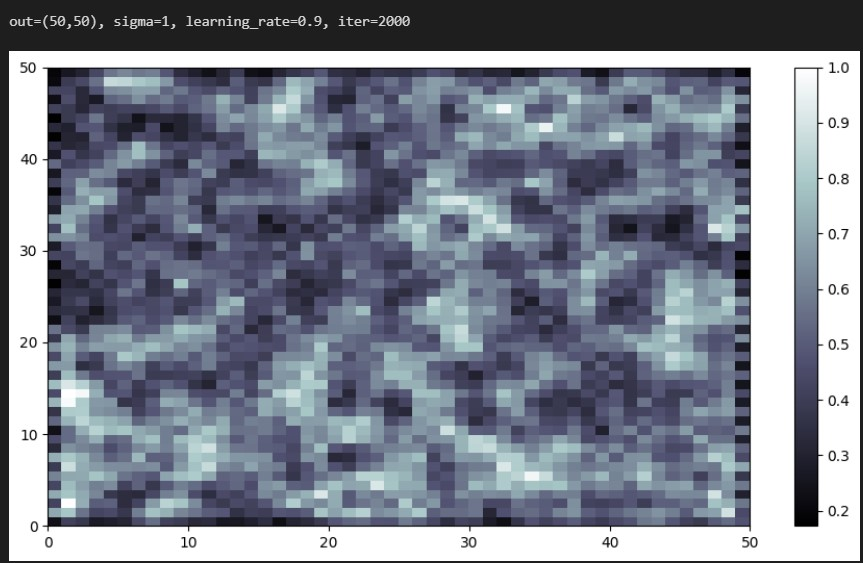
\includegraphics[scale=.65]{./p3-1}
    \caption{ماتریس یو با مشخصات داخل تصویر}\label{fig.31}
\end{figure}

\begin{figure}[!h]
    \centering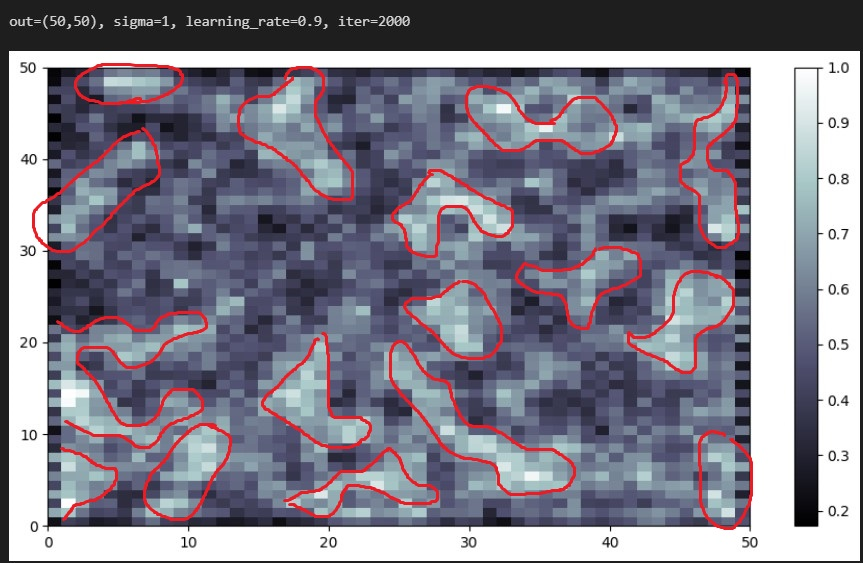
\includegraphics[scale=.65]{./p3-2}
    \caption{ماتریس یو با مشخصات داخل تصویر}\label{fig.32}
\end{figure}


\cleardoublepage

\begin{figure}[!h]
    \centering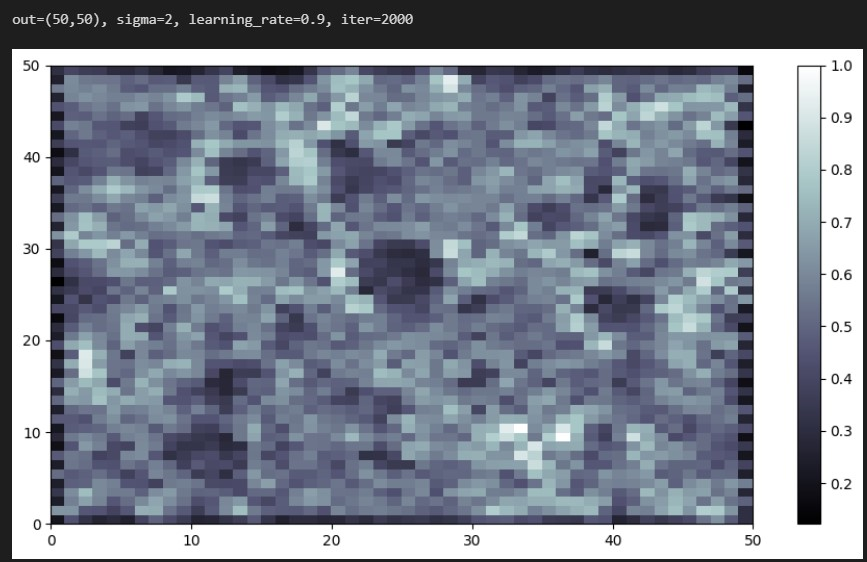
\includegraphics[scale=.65]{./p3-3}
    \caption{ماتریس یو با مشخصات داخل تصویر}\label{fig.33}
\end{figure}

\begin{figure}[!h]
    \centering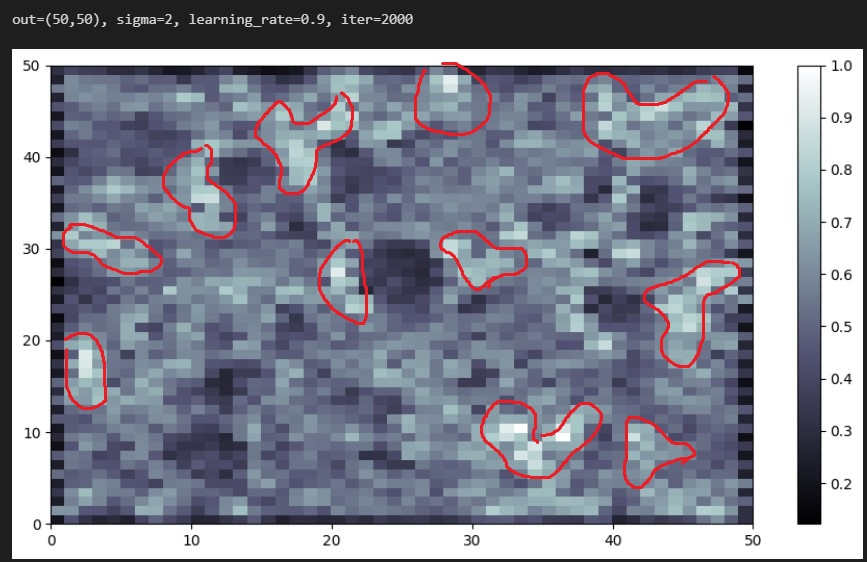
\includegraphics[scale=.65]{./p3-4}
    \caption{ماتریس یو با مشخصات داخل تصویر}\label{fig.34}
\end{figure}


\cleardoublepage

\begin{figure}[!h]
    \centering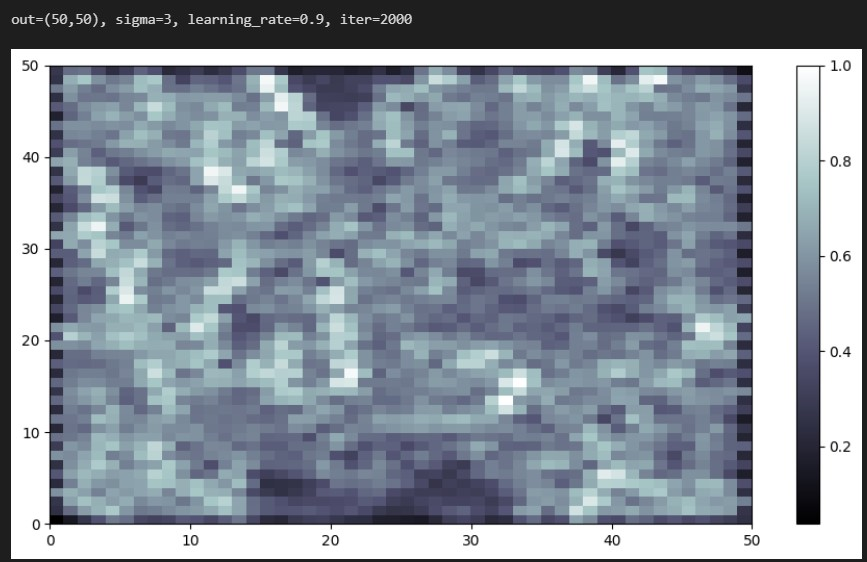
\includegraphics[scale=.65]{./p3-5}
    \caption{ماتریس یو با مشخصات داخل تصویر}\label{fig.35}
\end{figure}

\begin{figure}[!h]
    \centering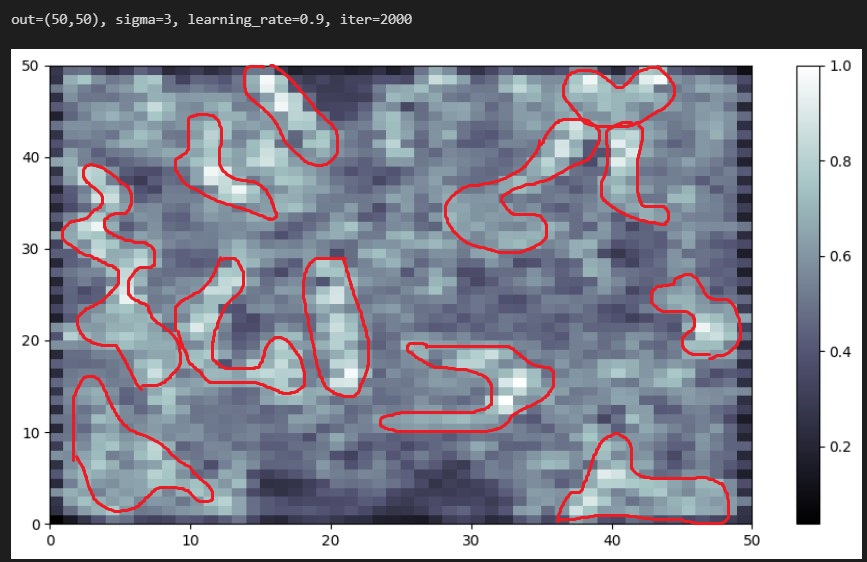
\includegraphics[scale=.65]{./p3-6}
    \caption{ماتریس یو با مشخصات داخل تصویر}\label{fig.36}
\end{figure}


\cleardoublepage

\begin{figure}[!h]
    \centering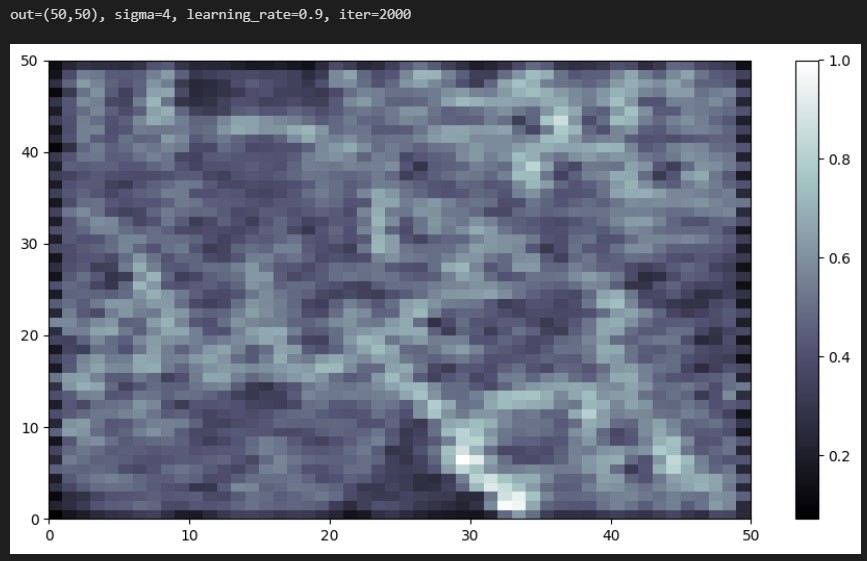
\includegraphics[scale=.65]{./p3-7}
    \caption{ماتریس یو با مشخصات داخل تصویر}\label{fig.37}
\end{figure}

\begin{figure}[!h]
    \centering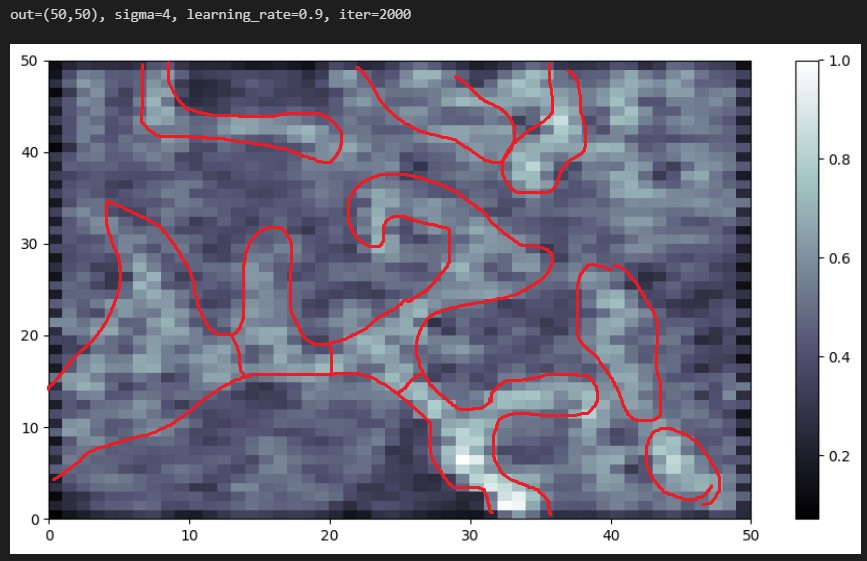
\includegraphics[scale=.65]{./p3-8}
    \caption{ماتریس یو با مشخصات داخل تصویر}\label{fig.38}
\end{figure}


\cleardoublepage


\begin{figure}[!h]
    \centering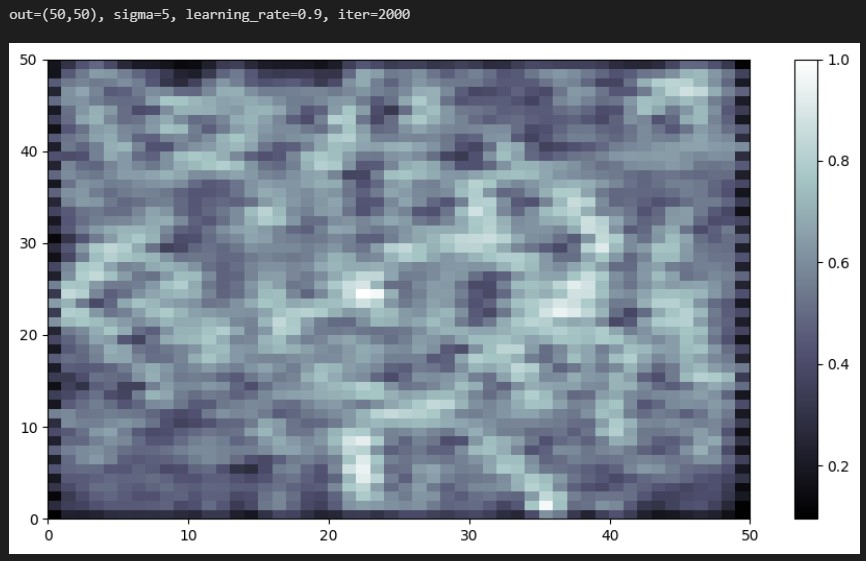
\includegraphics[scale=.65]{./p3-9}
    \caption{ماتریس یو با مشخصات داخل تصویر}\label{fig.39}
\end{figure}

\begin{figure}[!h]
    \centering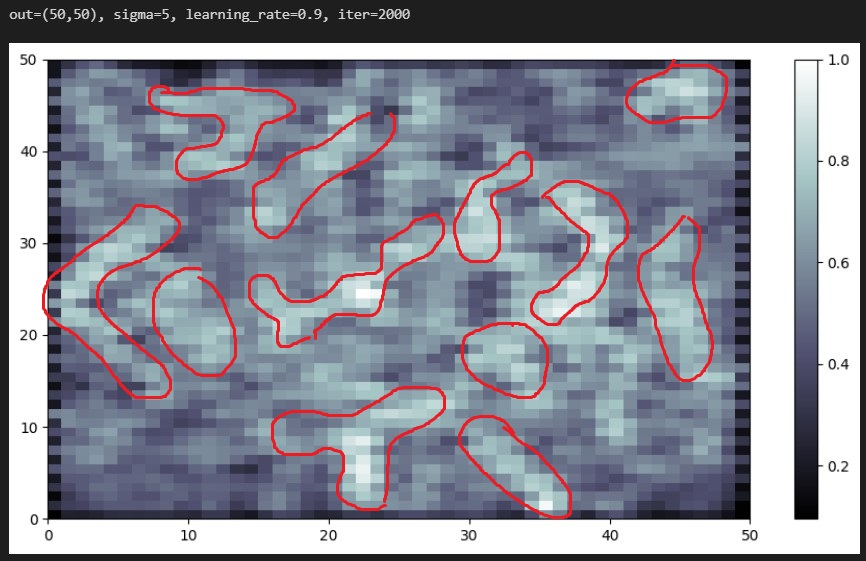
\includegraphics[scale=.65]{./p3-10}
    \caption{ماتریس یو با مشخصات داخل تصویر}\label{fig.310}
\end{figure}


\cleardoublepage


\begin{figure}[!h]
    \centering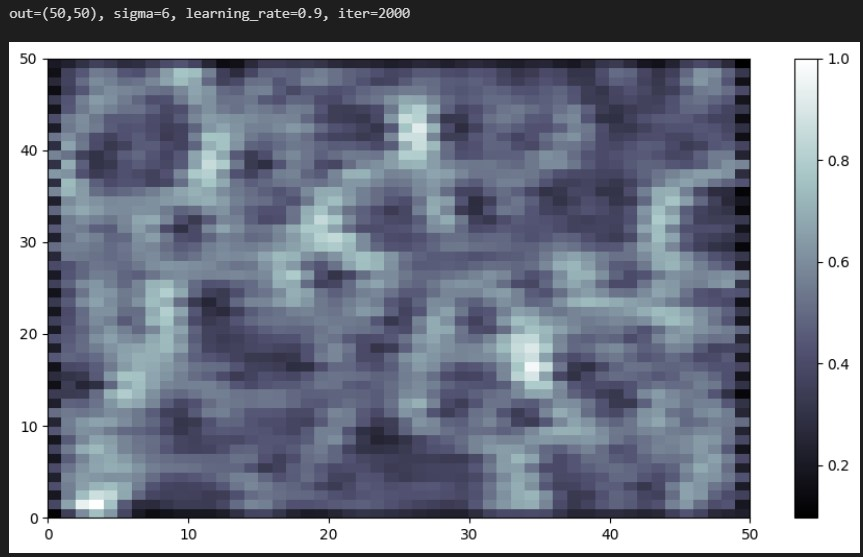
\includegraphics[scale=.65]{./p3-11}
    \caption{ماتریس یو با مشخصات داخل تصویر}\label{fig.311}
\end{figure}

\begin{figure}[!h]
    \centering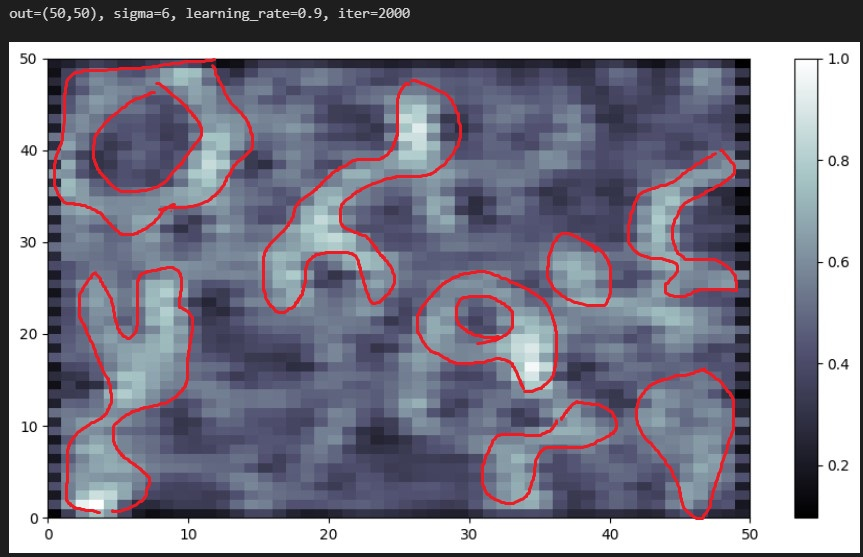
\includegraphics[scale=.65]{./p3-12}
    \caption{ماتریس یو با مشخصات داخل تصویر}\label{fig.312}
\end{figure}


\cleardoublepage


\begin{figure}[!h]
    \centering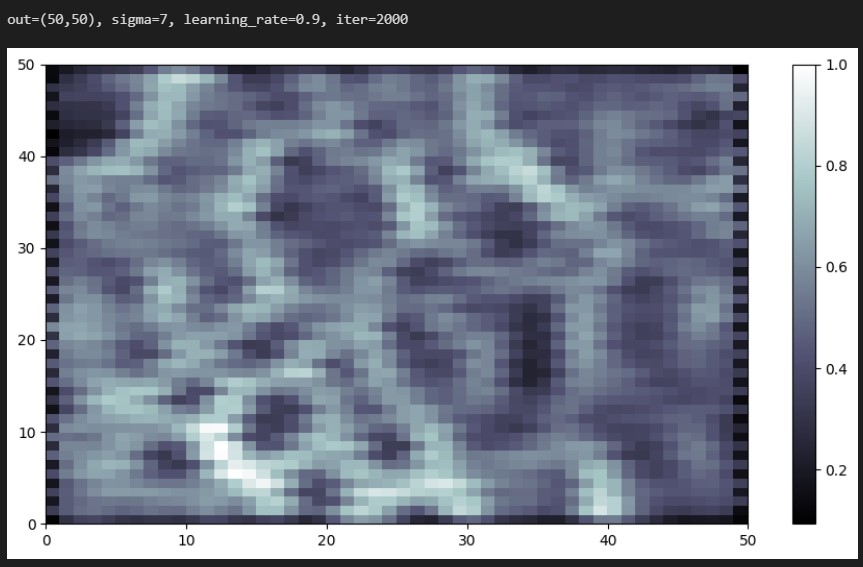
\includegraphics[scale=.65]{./p3-13}
    \caption{ماتریس یو با مشخصات داخل تصویر}\label{fig.313}
\end{figure}

\begin{figure}[!h]
    \centering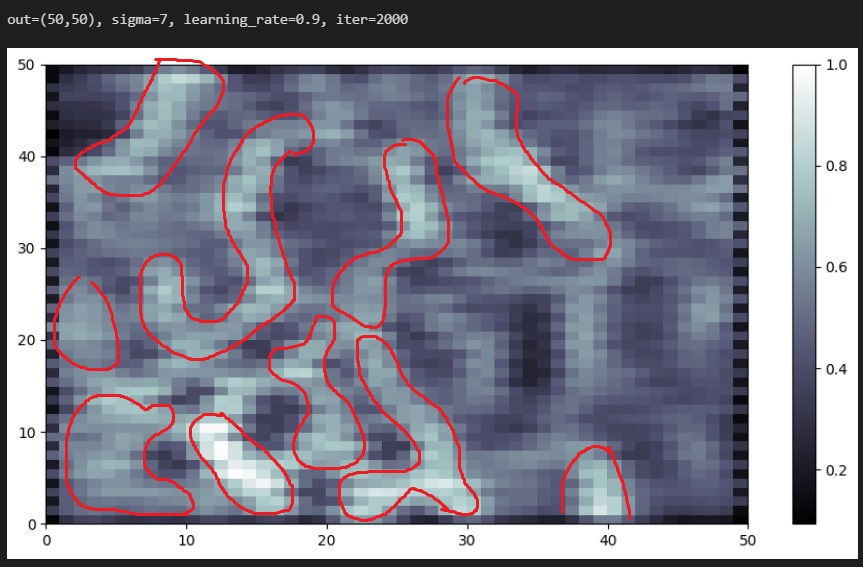
\includegraphics[scale=.65]{./p3-14}
    \caption{ماتریس یو با مشخصات داخل تصویر}\label{fig.314}
\end{figure}


\cleardoublepage

همانطور که مشاهده شد، تعداد خوشه‌ها از 8 تا 16 متغیر بود. و برای این‌ که مقدار امنی برای تعداد خوشه‌ها در نظر بگیریم. فرض می‌کنیم که لایه خروجی شامل 16 نورون (4 در 4) خواهد بود. 


% -------------------------------------------------------------------
\section{سوال دوم - ج}

یک روش اولیه این خواهد بود که از الگوریتم‌های خوشه‌بندی بر روی خود ماتریس یو استفاده کنیم (مثل \lr{DBSCAN}). بدین صورت می‌توانیم خوشه‌ها و قسمت‌های شبیه به هم ماتریس یو و سپس خوشه‌های مسئله و بعد نهایی شبکه را بدست آوریم.

اما اگر نخواهیم از ماتریس یو استفاده کنیم، روش دیگر استفاده از \lr{gsom} خواهد بود. این شبکه با حداقل تعداد گره (معمولا 4) شروع می‌شود و گره‌های جدید را بر اساس اکتشافی در مرز اضافه می‌کند. با استفاده از مقداری به نام عامل گسترش (\lr{SF})، این اتفاق می‌افتد. تمام گره های شروع، گره‌های مرزی هستند، یعنی هر گره آزادی دارد که در ابتدا در جهت خود رشد کند. گره های جدید از گره‌های مرزی رشد می‌کنند. هنگامی که یک گره برای رشد انتخاب شد، تمام موقعیت‌های مجاور آزاد آن، گره های جدید رشد خواهند کرد. همانطور که ذکر شد این شبکه به صورت پویا رشد می‌کند. از آنجایی که نیازی به از پیش تعیین ساختار شبکه نیست، می‌توان از تشکیل خوشه‌های پیش از موعد نیز به جای سازماندهی در یک خوشه مناسب جلوگیری کرد.


% -------------------------------------------------------------------
\section{سوال دوم - د}

حال فرض می‌کنیم که 10 خوشه داریم. برای طراحی شبکه‌ای مناسب، فرض می‌کنیم که طول و عرض شبکه باهم برابر است، یعنی شبکه‌هایی با ابعاد 3 در 3 یا 4 در 4 (با توجه به 10 خوشه). که شبکه با ابعاد 4 در 4 مناسب 10 خوشه خواهد بود.


در ادامه ماتریس یو برای این شبکه آورده شده است (سیگما (1)، تکرار (10000)، ابعاد شبکه (4 در 4)).

\begin{figure}[!h]
    \centering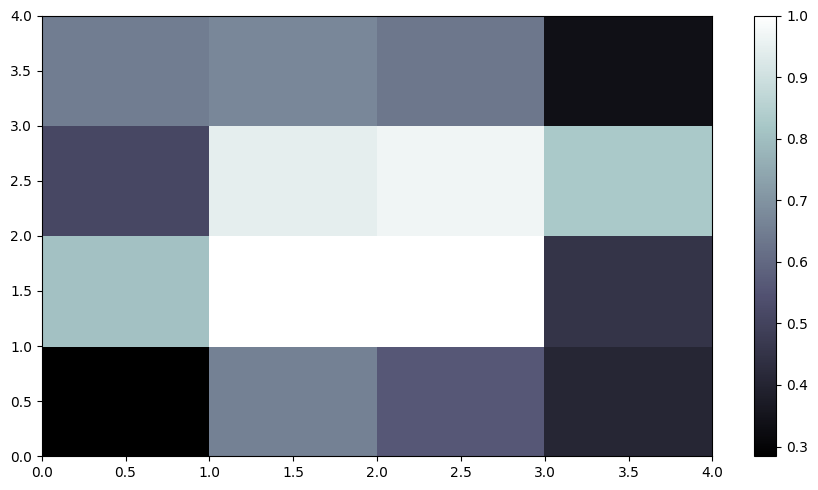
\includegraphics[scale=.65]{./p6-1}
    \caption{ماتریس یو با مشخصات داخل تصویر}\label{fig.61}
\end{figure}
\cleardoublepage

\begin{figure}[!h]
    \centering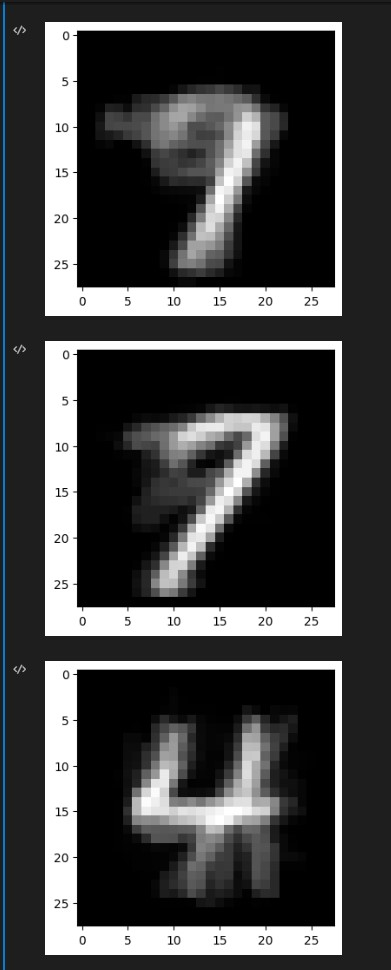
\includegraphics[scale=.65]{./p6-2}
    \caption{کلاس غالب سلول‌ها}\label{fig.62}
\end{figure}

\begin{figure}[!h]
    \centering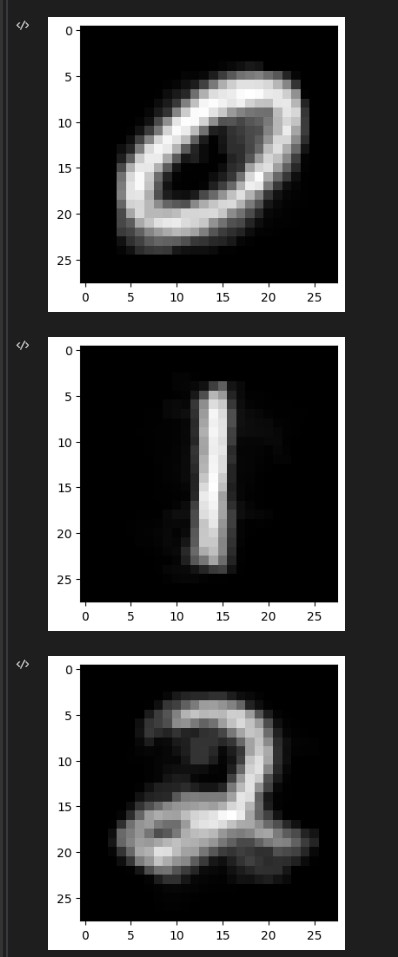
\includegraphics[scale=.65]{./p6-3}
    \caption{کلاس غالب سلول‌ها}\label{fig.63}
\end{figure}

\begin{figure}[!h]
    \centering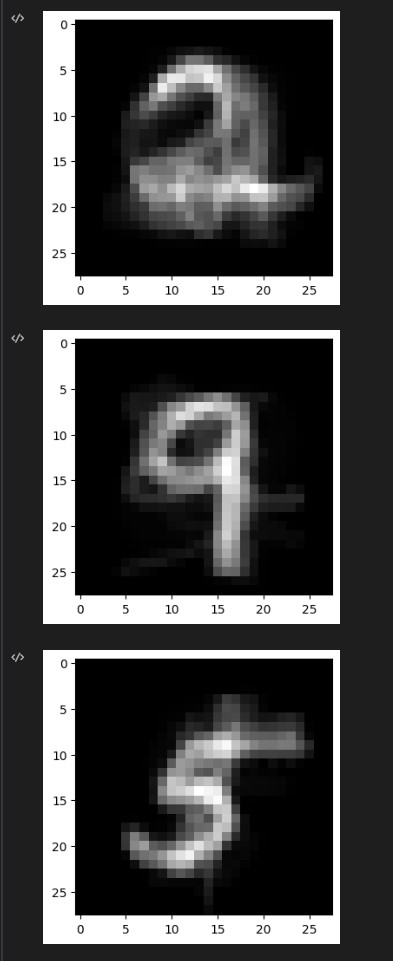
\includegraphics[scale=.65]{./p6-4}
    \caption{کلاس غالب سلول‌ها}\label{fig.64}
\end{figure}

\begin{figure}[!h]
    \centering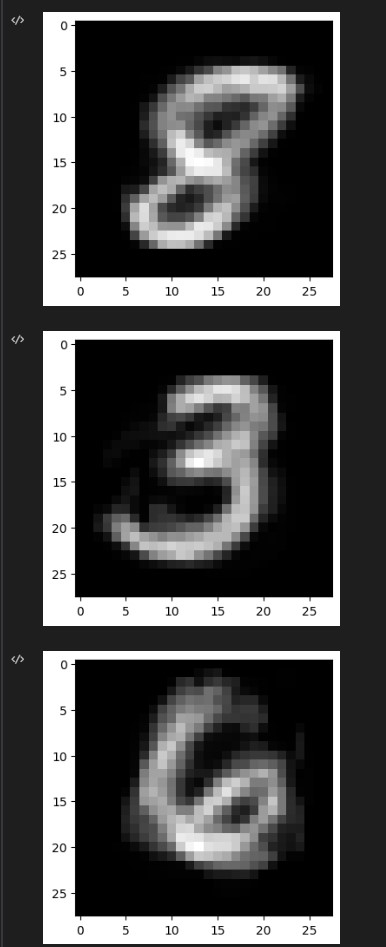
\includegraphics[scale=.65]{./p6-5}
    \caption{کلاس غالب سلول‌ها}\label{fig.65}
\end{figure}

\begin{figure}[!h]
    \centering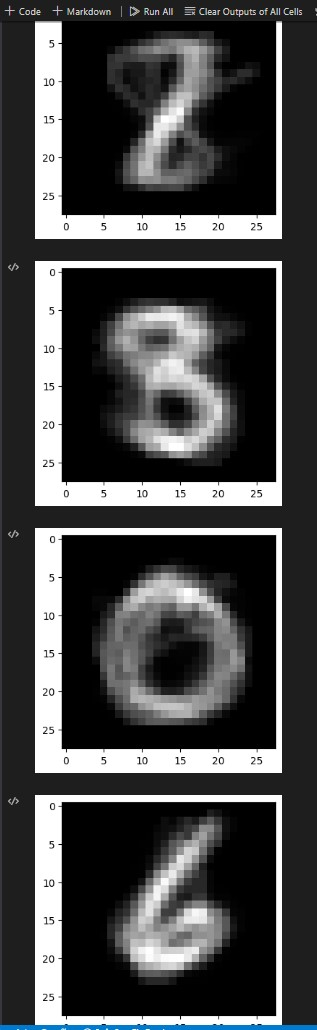
\includegraphics[scale=.65]{./p6-6}
    \caption{کلاس غالب سلول‌ها}\label{fig.66}
\end{figure}

\cleardoublepage

همانطور که مشاهده می‌شود با 6 خوشه اضافه تمام 10 کلاس موجود شناسایی شدند (مراکز خوشه).
همچنین خروجی سوال ب که شبکه‌ای با ابعاد 4 در 4 بود نیز در اینجا مورد استفاده قرار گرفت.


% -------------------------------------------------------------------

\end{document}